\documentclass{beamer}

% Theme for the presentation
\usetheme{Madrid}  % You can change the theme (e.g., AnnArbor, Berlin, etc.)

% Optional colors
\usecolortheme{dolphin}  % You can change this as well

% Packages to include if needed
\usepackage{graphicx} % For including images
\usepackage{amsmath, amssymb} % For mathematical symbols
\usepackage{hyperref} % For clickable links

% Title Page Info
\title[Weekly Presentation]{Weekly Presentation}
\subtitle{Group 3}
\author{Jessica Fornetti, Anais Blenet, Saul Burgess, Kaustubh Trivedi, Yuanshuo Du, Andreas Kraus}
\institute{TU Dublin}
\date{23rd of September, 2024} % You can specify a fixed date if needed

% Begin document
\begin{document}

% Title Slide
\begin{frame}
    \titlepage{}
\end{frame}

% Section 1
\section{Introduction}

% Problem desc Slide
\begin{frame}{Problem description}  % Slide title
    \begin{description}
        \item[1:] To help enhance the efficiency of urban planning for public authorities by providing detailed insight into available amenities
        \item[2:] Amenities include and are not limited to parking spaces (formal and informal), bike sheds, accessible ramps, bike lanes, etc
        \item[3:] This enhancement will be achieved through the development of a prototype Single Page Application (SPA) that integrates computer vision with publicly available mapping datasets 
        \item[4:] The area of interest will be Dublin city 
    \end{description}
\end{frame}

\begin{frame}{Overview of the System}
    \begin{figure}
        \centering
        \includegraphics[width=1\textwidth]{System_Diagram.png}
        \caption{System Diagram}
        \label{fig:system_diagram}
    \end{figure}
\end{frame}

% Use cases & users Slide
\begin{frame}{Use cases and Users}
    \begin{itemize}
        \item We will be focusing on parking amenities.
        \item Potential users and their associated use cases:
        \begin{itemize}
            \item \textbf{1. Civil servants} - for urban planning purposes such as:
            \begin{itemize}
                \item ensuring parking spaces adhere to local zoning regulations
                \item assessing the demand/supply for parking in various areas of a city
                \item overseeing existing parking amenities, conditions, and pricing
                \item considering environmental and traffic impact when planning to build new spaces
            \end{itemize}
            \item \textbf{2. Private Individuals} - for personal use in the following scenarios:
            \begin{itemize}
                \item viewing real-time parking availability given their current location or a specified destination within a defined radius
                \item seeing the cost of available parking spots nearby allowing users to compare and choose the best option
                \item viewing available parking based on special filters, such as handicap-accessible parking, electric vehicle charging stations, etc.
            \end{itemize}
        \end{itemize}
    \end{itemize}
\end{frame}

\begin{frame}{Use Case Diagram}
    \begin{figure}
        \centering
        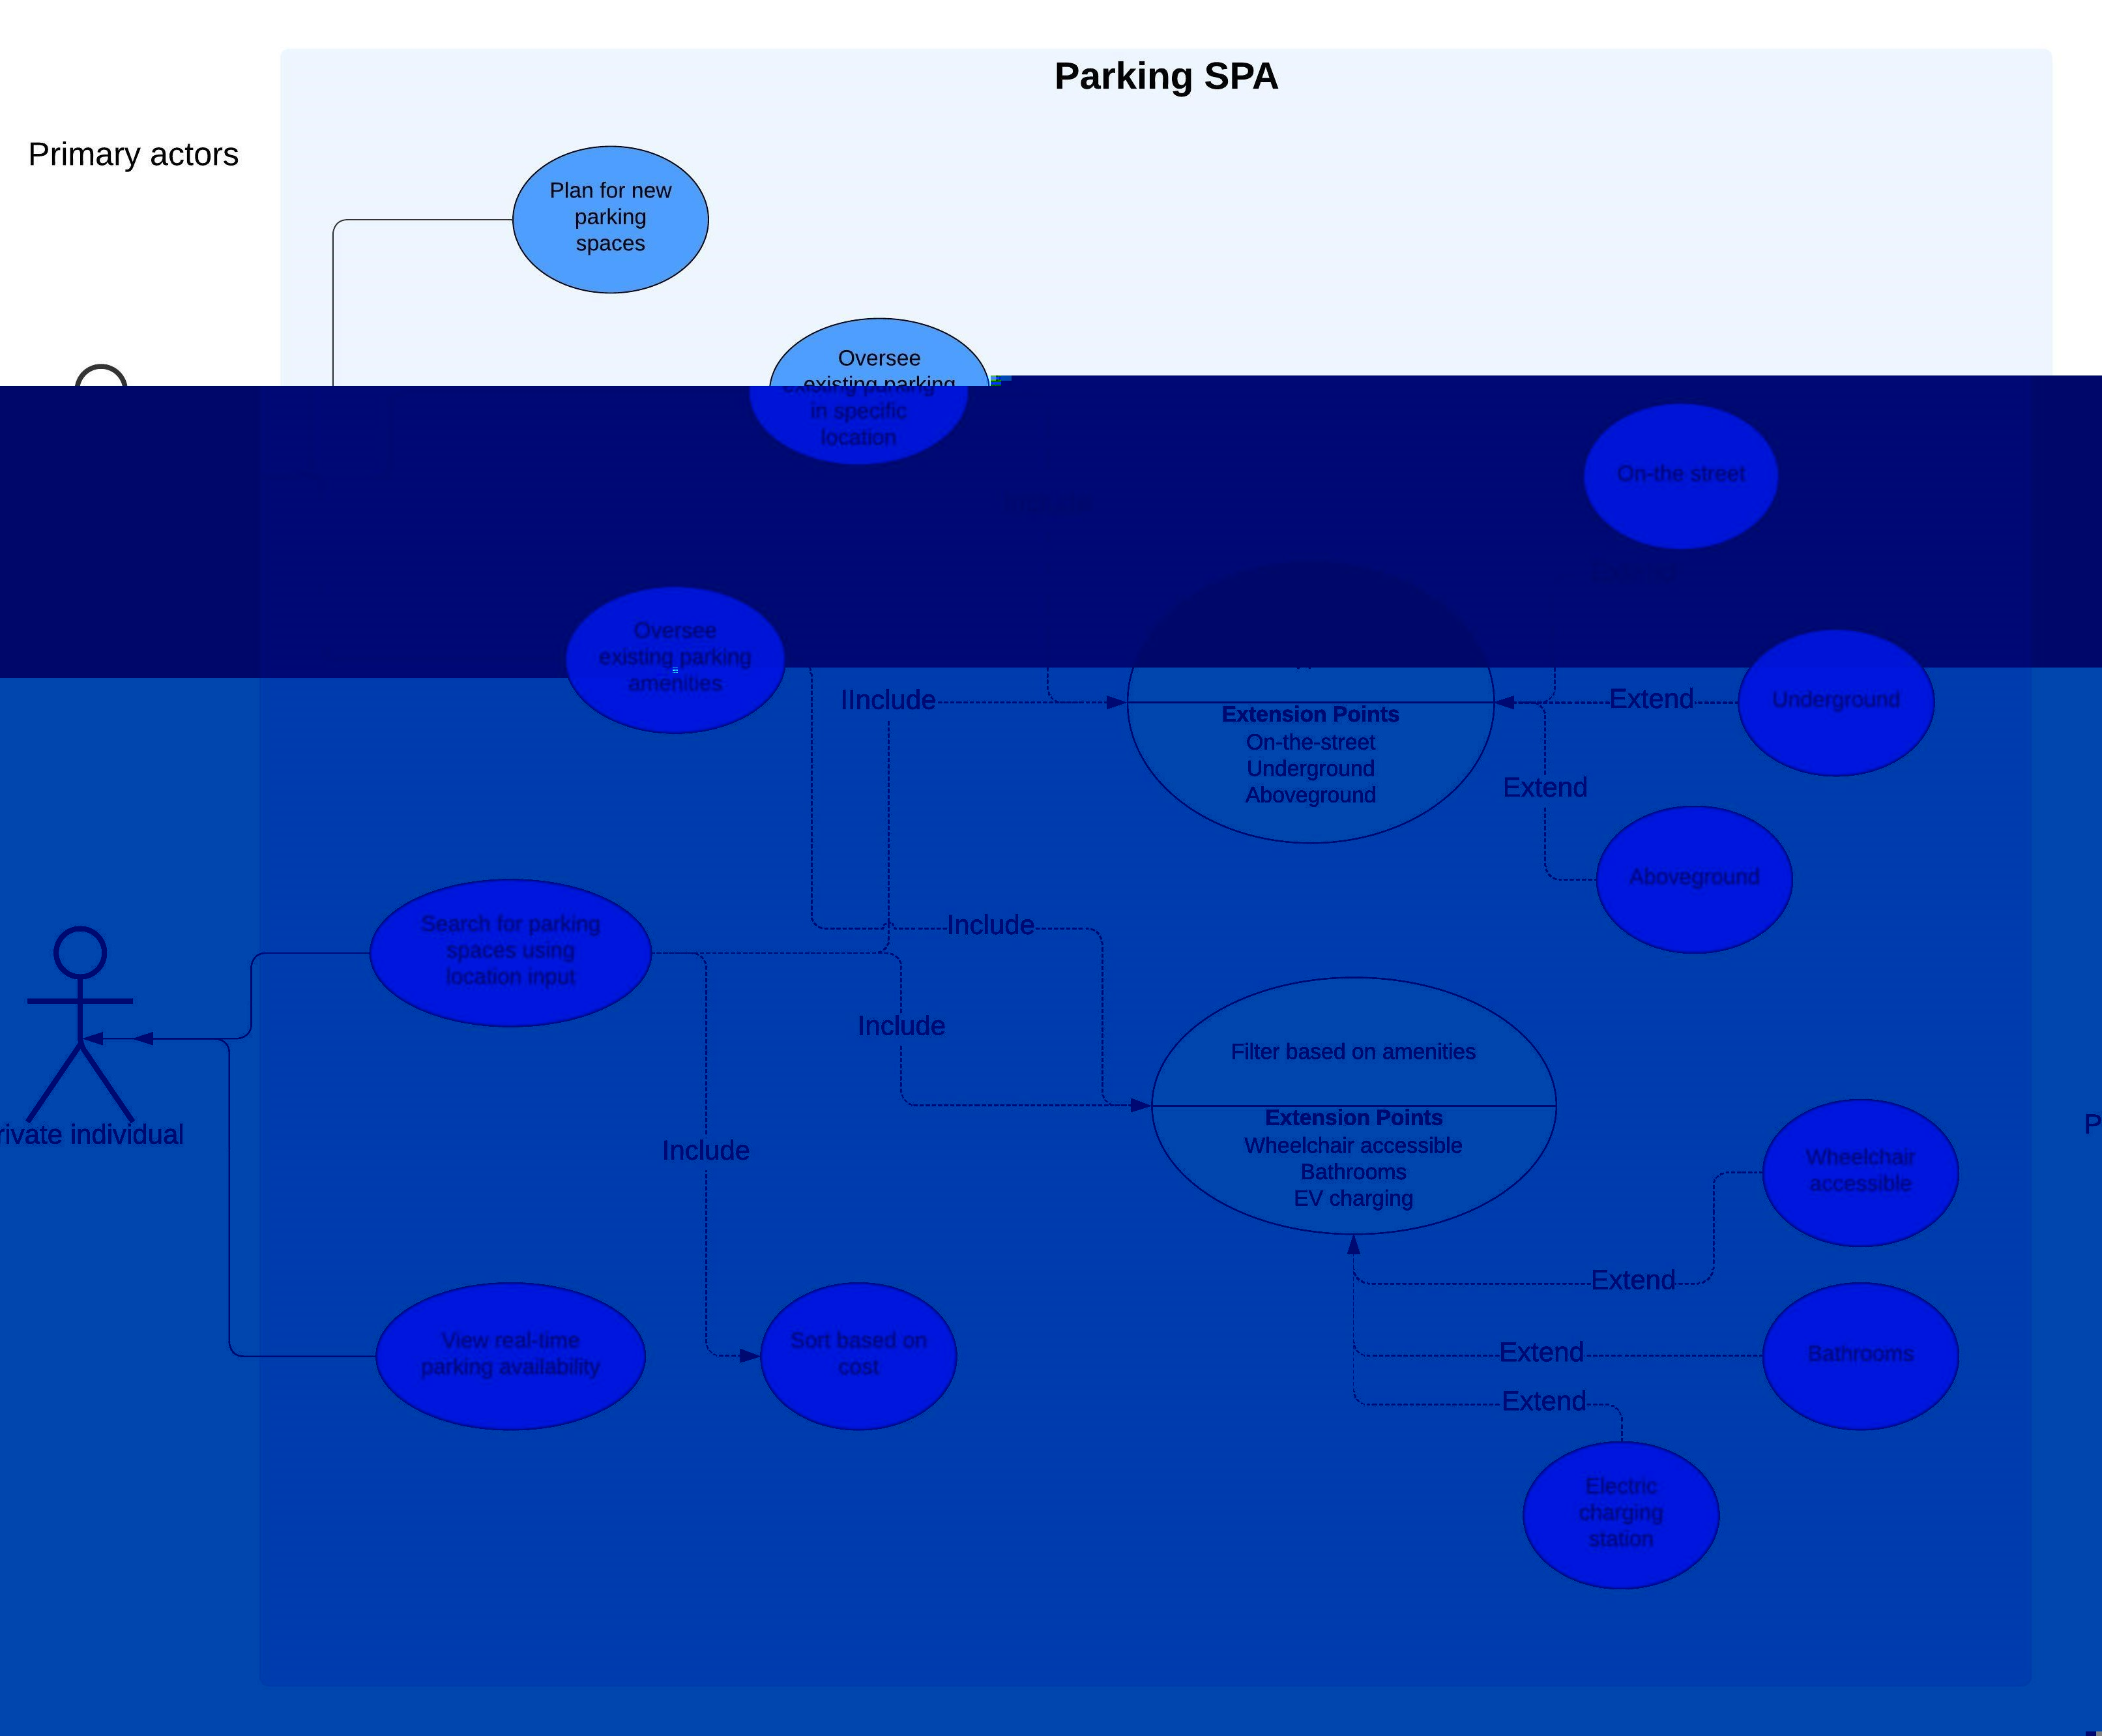
\includegraphics[width=0.8\textwidth]{Use_case_diagram_Parking_SPA.jpeg}
        \caption{Use Case Diagram}
        \label{fig:use_case_diagram}
    \end{figure}
\end{frame}


% Section 2
\section{Main Content}
\subsection{Approaches}
% Different Approaches Slide
\begin{frame}{Different Approaches}
    \begin{itemize}
        \item{Machine Learning Techniques : Convolutional Neural Networks}
        \item{Integration of Geospatial Data with Public Records}
        \item{Web Based Applications}
    \end{itemize}
\end{frame}

% Different Approaches Slide 2
\begin{frame}{Different Approaches: Convolutional Neural Networks}
    \begin{itemize}
        \item{Data Preparation : Preprocessing Steps}
        \begin{itemize}
        \item{Image Segmentation}
        \item{Noise Reduction}
        \item{Normalization}
        \end{itemize}
        \item{Model Training }
        \begin{itemize}
        \item{Different architectures}
        \item{Hyperparameter Tunning}
        \item{Regularization Techniques}
        \end{itemize}
        \item{Validation and Testing}
    \end{itemize}
\end{frame}

% Different Approaches Slide 3
\begin{frame}{Integration of Geospatial Data with Public Records}
    \begin{itemize}
        \item{Data Fusion}
        \item{Geospatial Analysis }
        \begin{itemize}
        \item{Measure Distances}
        \item{Identify Service Zones}
        \item{Identify Facility Clusters }
        \end{itemize}
        \item{GIS Tools}
    \end{itemize}
\end{frame}

% Different Approaches Slide 4
\begin{frame}{Web Based Applications}
    \begin{itemize}
        \item{User Interface Design}
        \item{Back-End Development}
        \begin{itemize}
        \item{Create Database}
        \item{Preprocess datasets}
        \item{Implement Machine Learning models}
        \end{itemize}
        \item{Scalability and Security}
    \end{itemize}
\end{frame}


\subsection{Design and build}
% Design & build Slide 5
\begin{frame}{Design and Build} We will focus on the parking amenity first, and proceed in 3 phases:
    \begin{itemize}
        \item{\textbf{1. Model training} - }Training and developing a convolutional neural network (CNN) to distinguish street-level parking spaces from aerial images.
        \item{\textbf{2. Map creation} - } Developing a user-friendly mapping interface that allows users to choose a particular location and view the availability of street-level parking in the vicinity of that location.
        \item{\textbf{3. Integrating data sources} - } Integrating additional information sources to include formal parking spaces (under and aboveground, etc)
    \end{itemize}
\end{frame}

% Design & build: Phase 1 Slide 6
\begin{frame}{Design and Build: Phase 1 - Model training}
    \begin{itemize}
        \item{\textbf{1. Data Collection and Preparation} - } High resolution aerial photographs will be gathered from multiple public sources. These images will undergo preprocessing to enhance their quality and consistency such as noise reduction, normalization, and image segmentation.
        \item{\textbf{2. Model Development and Training} - } A CNN will be trained on the preprocessed image to recognize street-level parking areas. Different architectural configurations will be used and hyperparameter tuning will be performed to optimize the model's accuracy and reduce overftitting.
        \item{\textbf{3.Validation and Testing} - } The model will be tested using a separate validation dataset ensuring it performs well in different urban settings. Various performance metrics (accuracy, precision, recall) will be used to assess the model.
    \end{itemize}
\end{frame}

% Design & build: Phase 2 Slide 7
\begin{frame}{Design and Build: Phase 2 - Map creation}
    \begin{itemize}
        \item{\textbf{1. Interactive map development} - } Utilizing GIS software and web development frameworks- an interactive map will be created. Users will be able to choose any spot on the map to query the back-end for parking information in a vicinity of the area.
        \item{\textbf{2. Integration with ML model} - } The map interface will communicate with the back-end server where the CNN operates. When a user selects a location, the corresponding aerial image will be processed by the CNN to highlight available parking spaces.
        \item{\textbf{3. Front + Back-end integration} - }The SPA’s front-end will be developed using Next.js, while the back-end will utilize Go to handle API requests, process data, and return results to the user interface.
    \end{itemize}
\end{frame}

% Design & build: Phase 3 Slide 8
\begin{frame}{Design and Build: Phase 3 - Integrating data sources}
    \begin{itemize}
        \item{\textbf{1. Data integration} - }Data concerning underground parking facilities will be sourced from municipal records and other relevant databases. This information will be fused with the aerial image analysis to offer a holistic view of parking availability.
        \item{\textbf{2. System enhancement} - }Data fusion techniques will be employed to ensure seamless integration of information sources.
        \item{\textbf{3. UI expansion} - }The existing SPA interface will be enhanced to display not just street-level but also underground parking options, allowing users to make more informed decisions based on a comprehensive visualization.
    \end{itemize}
\end{frame}

% Design & build: Phase 3 Slide 9 (references)
\begin{frame}{References}
    \begin{itemize}
        \item Abidin, Muhammad Zainal and Reza Pulungan (2020). “A systematic review of machine-vision-based smart parking systems”. In: Sci. J. Informatics 7.2, pp. 213–227.
        \item Gopinath, B et al. (2023). “Deep Learning based Automated Parking Lot Space Detection using Aerial Imagery”. In: 2023 2nd International Conference on Advancements in Electrical, Electronics, Communication, Computing and Automation (ICAECA). IEEE, pp. 1–4.
        \item Grbić, Ratko and Brando Koch (2023). “Automatic vision-based parking slot detection and occupancy classification”. In: Expert systems with applications 225, p. 120147.
        \item Iqbal, Kashif et al. (2021). “Autonomous Parking-Lots Detection with Multi-Sensor Data Fusion Using Machine Deep Learning Techniques.” In: Computers, Materials, Continua 66.3.
        \item Li, Yongyi et al. (2022). “Research on Parking Space Status Recognition Method Based on Computer Vision”. In: Sustainability 15.1, p. 107.
    \end{itemize}
\end{frame}

\end{document}
